\documentclass[border=10pt]{standalone}
\usepackage[svgnames]{xcolor}
\usepackage{amsmath}
\usepackage{pgfplots}
\pgfplotsset{compat=newest}
\usepackage[sfdefault]{FiraSans}
\usepackage{FiraMono}
\renewcommand*\familydefault{\sfdefault}
\begin{document}
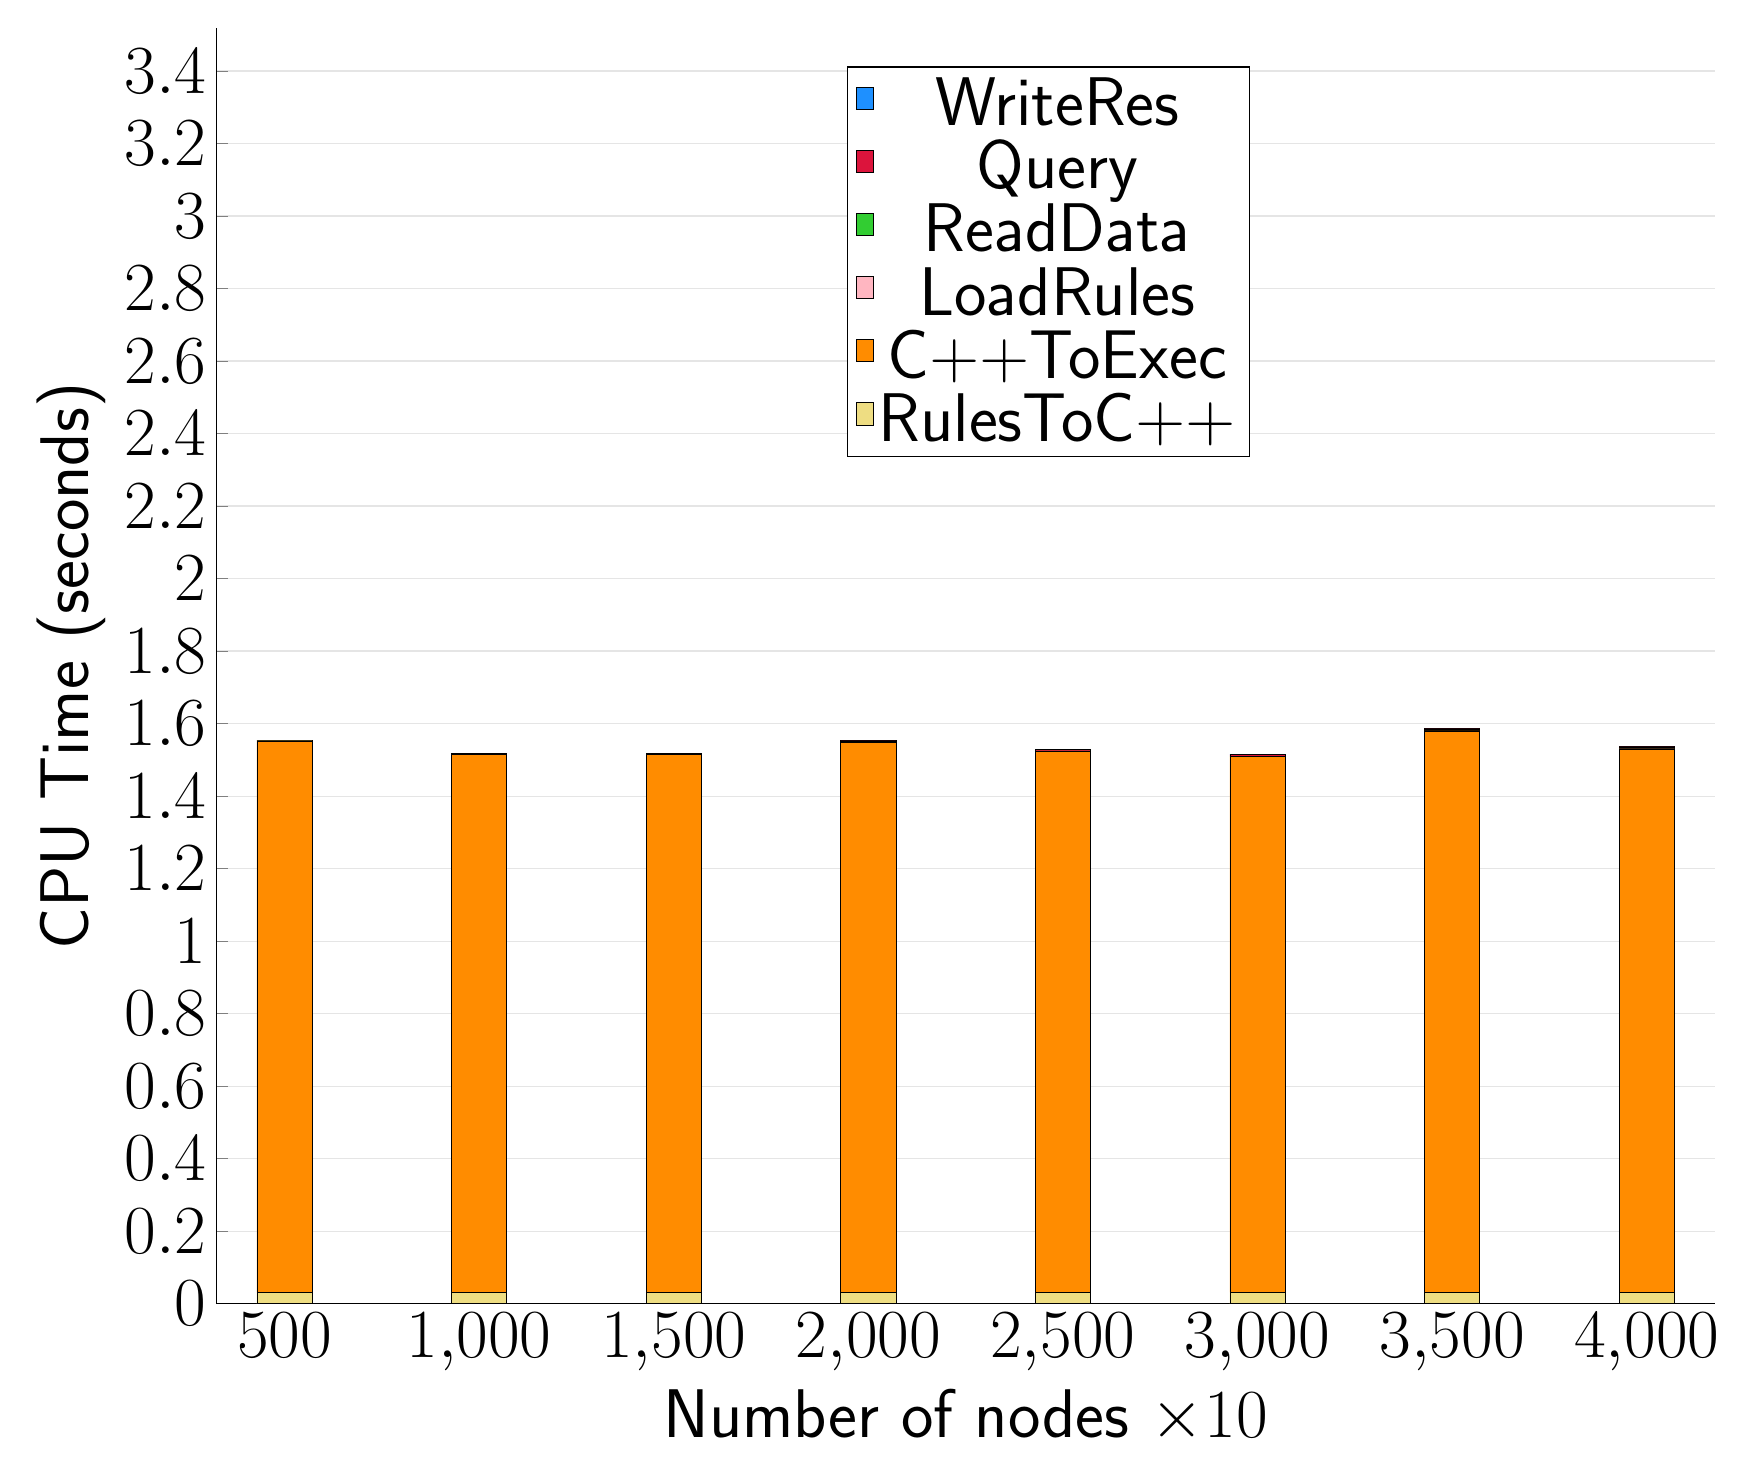
\begin{tikzpicture}
\begin{axis}[
   ybar stacked,
   width=1.7\textwidth,
   bar width=0.7cm,
   ymajorgrids, tick align=inside,
   major grid style={draw=gray!20},
   xtick=data,
   ymin=0, ymax=3.518,
   axis x line*=bottom,
   axis y line*=left,
   enlarge x limits=0.05,
   legend style={
       at={(0.69, 0.97)},
       anchor=north east,
       legend columns=1,
       font=\Huge,
   },
   ylabel={CPU Time (seconds)},
   xlabel={Number of nodes $\times 10$},
   label style={font=\Huge},
   tick label style={font=\Huge},
]
\addlegendimage{fill=DodgerBlue, draw=black, line width=0.2pt}
\addlegendentry{WriteRes}
\addlegendimage{fill=Crimson, draw=black, line width=0.2pt}
\addlegendentry{Query}
\addlegendimage{fill=LimeGreen, draw=black, line width=0.2pt}
\addlegendentry{ReadData}
\addlegendimage{fill=LightPink, draw=black, line width=0.2pt}
\addlegendentry{LoadRules}
\addlegendimage{fill=DarkOrange, draw=black, line width=0.2pt}
\addlegendentry{C++ToExec}
\addlegendimage{fill=LightGoldenrod, draw=black, line width=0.2pt}
\addlegendentry{RulesToC++}
\addplot +[fill=LightGoldenrod, draw=black, line width=0.2pt] coordinates {
(500, 0.030000000000000006)
(1000, 0.030000000000000006)
(1500, 0.030000000000000006)
(2000, 0.03200000000000001)
(2500, 0.030000000000000006)
(3000, 0.031000000000000007)
(3500, 0.030000000000000006)
(4000, 0.030000000000000006)
};
\addplot +[fill=DarkOrange, draw=black, line width=0.2pt] coordinates {
(500, 1.522)
(1000, 1.4849999999999999)
(1500, 1.485)
(2000, 1.517)
(2500, 1.4940000000000002)
(3000, 1.4780000000000002)
(3500, 1.55)
(4000, 1.5000000000000002)
};
\addplot +[fill=LightPink, draw=black, line width=0.2pt] coordinates {
(500, 9.460000000000001e-05)
(1000, 8.35e-05)
(1500, 0.0001245)
(2000, 0.0001095)
(2500, 0.0001096)
(3000, 0.0001107)
(3500, 0.00010599999999999997)
(4000, 9.38e-05)
};
\addplot +[fill=LimeGreen, draw=black, line width=0.2pt] coordinates {
(500, 0.00036219999999999997)
(1000, 0.000438)
(1500, 0.0006209)
(2000, 0.0006962)
(2500, 0.0007963999999999998)
(3000, 0.0009488999999999999)
(3500, 0.0009544999999999999)
(4000, 0.0010449)
};
\addplot +[fill=Crimson, draw=black, line width=0.2pt] coordinates {
(500, 0.0005748999999999999)
(1000, 0.0011323)
(1500, 0.0019804999999999996)
(2000, 0.0024635)
(2500, 0.0032034)
(3000, 0.0040076)
(3500, 0.004196200000000001)
(4000, 0.0047366)
};
\addplot +[fill=DodgerBlue, draw=black, line width=0.2pt] coordinates {
(500, 0.00044130000000000005)
(1000, 0.0006418)
(1500, 0.000941)
(2000, 0.0011699999999999998)
(2500, 0.0014166)
(3000, 0.0017017)
(3500, 0.0017325)
(4000, 0.0019244999999999998)
};
\end{axis}
\end{tikzpicture}

\end{document}
